\documentclass[12pt, letterpaper]{article}
\usepackage[titletoc,title]{appendix}
\usepackage{color}
\usepackage{booktabs}
\usepackage[usenames,dvipsnames,svgnames,table]{xcolor}
\definecolor{dark-red}{rgb}{0.75,0.10,0.10} 
\definecolor{dark-blue}{rgb}{0.0,0.0,0.7} 
\usepackage[margin=1in]{geometry}
\usepackage[linkcolor=dark-blue,
			colorlinks=true,
			urlcolor=blue,
			pdfstartview={XYZ null null 1.00},
			pdfpagemode=UseNone,
			citecolor={dark-blue},
			pdftitle={Propagation of Error}]{hyperref}
%\usepackage{biblatex}
\usepackage{multibib}
\newcites{sec}{Other Sources}
\usepackage{geometry} % see geometry.pdf on how to lay out the page. There's lots.
\geometry{letterpaper}               % This is 8.5x11 paper. Options are a4paper or a5paper or other... 
\usepackage{graphicx}                % Handles inclusion of major graphics formats and allows use of 
\usepackage{amsfonts,amssymb,amsbsy}
\usepackage{amsxtra}
\usepackage{natbib}
\usepackage{dcolumn}
\usepackage{longtable}
\usepackage{verbatim}
\setcitestyle{round,semicolon,aysep={},yysep={;}}
\usepackage{setspace}		     % Permits line spacing control. Options are \doublespacing, \onehalfspace
\usepackage{sectsty}		     % Permits control of section header styles
\usepackage{lscape}
\usepackage{fancyhdr}		     % Permits header customization. See header section below.
\usepackage{url}                     % Correctly formats URLs with the \url{} tag
\usepackage{fullpage}		%1-inch margins
\usepackage{multirow}
\usepackage{rotating}
\setlength{\parindent}{3em}

\usepackage{float}

\usepackage[T1]{fontenc}
\usepackage{bm}
\usepackage{libertine}
\usepackage{dcolumn}
\usepackage{chngcntr}

% Caption
\usepackage[hang, font=small,skip=0pt, labelfont={bf}]{caption}
\captionsetup[subtable]{font=small,skip=0pt}
\usepackage{subcaption}

% tt font issues
% \renewcommand*{\ttdefault}{qcr}
\renewcommand{\ttdefault}{pcr}

\usepackage{lscape}
\renewcommand{\textfraction}{0}
\renewcommand{\topfraction}{0.95}
\renewcommand{\bottomfraction}{0.95}
\renewcommand{\floatpagefraction}{0.40}
\setcounter{totalnumber}{5}
\makeatletter
\providecommand\phantomcaption{\caption@refstepcounter\@captype}
\makeatother
\begin{comment}

setwd(paste0(githubdir, "propagation_of_error_dev/ms/"))
tools::texi2dvi("error.tex", pdf = TRUE, clean = TRUE) 
setwd(basedir)
  
\end{comment}

\begin{document}
\title{\Large{Propagation of Error: Approving Citations\\ to Problematic Research}\footnote{We are grateful to Danielle Portnoy and Xiaoran Huang for assisting us with research, and to Andrew Gelman, Kabir Khanna, and Daniel Stone for offering valuable comments. The data and scripts for replicating the analysis can be found at: \href{https://github.com/recite/propagation_of_error}{https://github.com/recite/propagation\_of\_error}}\\\vspace{5mm}}

\author{Ken Cor\thanks{Ken is Assistant Dean, Assessment in the Faculty of Pharmacy and Pharmaceutical Sciences at the University of Alberta, Edmonton. Ken can be reached at \href{mailto:mcor@ualberta.edu}{\tt{mcor@ualberta.edu}}} \and Gaurav Sood\thanks{Gaurav can be reached at \href{mailto:gsood07@gmail.com}{\tt{gsood07@gmail.com}}}
\vspace{5mm}}
\date{\normalsize{\today}}
\maketitle

\vspace{.2cm}
\doublespacing
\clearpage
\begin{abstract}
Many claims in a scientific article rest on research done by others. But when the claims are based on flawed research, scientific articles potentially spread misinformation. To shed light on how often scientists base their claims on problematic research, we exploit data on cases where problems with research are broadly publicized. Using data from over 3,000 retracted articles and over 74,000 citations to these articles, we find that at least 31.2\% of the citations to retracted articles happen a year after they have been retracted. And that 91.4\% of the post-retraction citations are \textit{approving}---note no concern with the cited article. We augment the analysis with data from an article published in \textit{Nature Neuroscience} highlighting a serious statistical error in articles published in prominent journals. Data suggest that problematic research was approvingly cited \textit{more frequently} after the problem was publicized. Our results have implications for the design of scholarship discovery systems and scientific practice more generally.
\end{abstract}

\clearpage

In April 2005, \citet{rubio2005spontaneous} published a disturbing finding in \textit{Cancer Research}. They reported discovering that stem cells can spontaneously transform into cancerous cells during \textit{in vitro} experiments. The finding was a blow to research in the use of stem cells to treat cancer. By 2010, according to \textit{Web of Science}, the article had been cited over 300 times.

In August 2010, the article was retracted \citep{de2010retraction}. The authors had been unable to replicate the results. Worse, there was mounting evidence that transformations like the one reported were due to a basic error in such research: cross-contamination during cell culturing. But the episode can be seen in a favorable light. Errors were caught, and information about the error was disseminated in the same venue where the original article was published. The story, however, does not end there.

Since retraction, the article has been cited another 300 plus times, with most citations not noting any concern with the original work. For instance, a year after retraction, \citet{firinci2011mesenchymal} published an article in \textit{International Immunopharmacology} citing \citeauthor{rubio2005spontaneous} as basis for warning scientists that stem cells can spontaneously transform. Two years after retraction, \citet{kosaka2012therapeutic} published an article in \textit{Cancer Gene Therapy} in which they cited spontaneous transformation of human cells into cancerous cells, crediting \citeauthor{rubio2005spontaneous} for the discovery, as a hurdle to implementation of treatment they find effective. Three years after retraction, \citet{chang2013safety} published an article in \textit{Aesthetic Plastic Surgery} citing \citeauthor{rubio2005spontaneous} as evidence against studies that suggest that spontaneous transformation of human stem cells is not a risk. As we find, these are not isolated examples. It is a pattern. 

In this paper, we study citations to research with serious errors. We tally how often research with serious errors is (approvingly) cited before and after the errors have been brought to light. To study the question, we exploit two datasets. The first dataset is a large original dataset of retracted articles---over 3,000 retracted articles and nearly 74,000 citations to retracted articles. The second dataset includes data from an article that highlights a potentially serious statistical error in articles published in prominent journals. Both sets of data suggest that articles with potentially serious errors continue to be cited approvingly long after the error has been publicized, either via a retraction notice or publication of an article noting the error. For instance, we find that at least 31.2\% of the citations to retracted articles happen a year after the publication of the retraction notice. And that 91.4\% of the post-retraction citations are \textit{approving}---note no concerns with the cited article. Our results have implications for the design of scholarship discovery systems, and for scientific practice more generally.

\section*{Potential Impact of Approvingly Citing Research With Serious Errors}

Citations are the bedrock of the scientific process. Scientists use citations to give credit for being first (``$x$, $y$, and $z$ have studied $a$''), to debate methods and inferences (``the method used in study $x$ fails to account for $s$''), as evidence (``$x$ shows $a$'', ``we use data from $x$ for our meta-analysis''), and to contextualize results (``our results are consistent with results from $y$''). And unless the researcher notes problems with cited research, citations cue that the data, results, inferences, or in some cases, the entire article, can be trusted.

When researchers \textit{approvingly} cite, i.e., note no concerns along with the citation, articles with serious errors, problems ensue. First, when erroneous research is approvingly cited as evidence \citep[e.g.,][]{chang2013safety, torsvik2010spontaneous}, it cues that the evidence for the claim is good. Such citations thus unduly increase the reader's confidence in the result or argument. When the claim being buffeted by the citation is wrong, such citations also misinform. In the extremum, a reader may become persuaded that the incorrect point is right. And such a reader, generally another academic, may go on to write other articles influenced by the incorrect point, citing the erroneous article for support, or may share the point as fact with colleagues and students, propagating the error.

Second, when erroneous research is approvingly cited to contextualize results \citep[e.g.,][]{kosaka2012therapeutic}, readers get a misleading impression of the plausibility of the numbers reported in the study.

Third, such citations give full credit to research (and researchers) when at best partial credit is deserved. And since citation tallies cue credibility, such citations make erroneous research appear yet more credible.\footnote{Even citations that note concerns with the retracted article will inflate the number of times a retracted article is cited. But when concerns are noted, better metrics can be built on top of the data. When no concern is noted, the task of building pro-rated metrics is considerably harder.}

Lastly, sometimes research is approvingly cited to acknowledge the source of the data. For instance, \citet{lin2013perioperative} used data from ``two retracted studies ... without acknowledgment of their retractions, both of which were for fraudulent data...'' \citep[p. 1][]{paul2015comment} in a meta-analysis. In such cases, the consequence is obvious and extreme---the key findings in the published work are incorrect.

In sum, \textit{approving} citations to problematic research propagate the error. 

\section*{Data, Research Design, and Expectations}
We expect approving citations to problematic research to stop once the problems have been made public. But some research suggests otherwise. For instance, research by John Darsee continued to be approvingly cited after a highly publicized retraction of his work \citep{kochan1992persistence}. Similarly, a study using a database of 235 retracted biomedical articles found that nearly 94\% of the citations after retraction treated research as valid \citep{budd1998phenomena}. Yet another study, exploiting a dataset of 82 retracted articles, came to similar conclusions \citep{pfeifer1990continued}.

All these studies, however, suffer from three weaknesses. First, the studies use small samples, often spanning a single discipline. Use of small, selective samples means that we still do not know how widespread the problem is. Second, the studies solely focus on citations after retraction. This means that we do not know how common approving citations are before the problems are publicized, and if the rate changes after publicity. And third, the studies only focus on retracted articles. Retraction is generally a result of serious scientific malpractice. By focusing on retractions alone, the studies fail to illuminate the much more common problem of approving citations to studies with major errors with potentially serious implications for the key results.

We address all three issues. We study approving citations to articles that make potentially serious errors that don't lead to a retraction by leveraging data from an article published in \textit{Nature} that highlights a potentially serious statistical error in articles published in prominent journals. To more extensively study approving citations to retracted articles, we assemble a large original dataset of retracted articles---over 3,000 retracted articles and nearly 74,000 citations to the retracted articles.

Our first dataset comes from an article that identifies articles that mistake the difference between a statistically significant and statistically insignificant result as evidence that the difference is statistically significant \citep{nieuwenhuis2011}. (For an explanation of why this is problematic, see \citet{gelman2006}.) \citet{nieuwenhuis2011} analyzed 170 articles published in \textit{Nature}, \textit{Science}, \textit{Neuron}, and \textit{Journal of Neuroscience} between 2009 and 2010. They found that roughly half of the 170 articles made this mistake. We used \href{https://webofknowledge.com}{Web of Science} (WoS) (we talk more about WoS below) \citep{reuters2012web} to download citations to all the 170 articles.

Our second dataset is a large novel dataset of retracted articles. We used WoS to assemble the data. WoS indexes articles from over 9,500 natural science journals and 3,500 social science journals \citep{yong2013web}. WoS indexes articles from over 12,000 international journals and 148,000 conferences \citep{yong2013web}. WoS contains key citation indices including the \textit{Science Citation Index Expanded} (over 9,500 journals; 1900--present), \textit{Social Sciences Citation Index} (over 3,500 journals; 1900--present), \textit{Arts \& Humanities Citation Index} (over 1,700 journals; 1975--present), \textit{Conference Proceedings Citation Index} (over 170,000 conferences; 1990-present), \textit{Book Citation Index} (over 30,000 titles; 2005--present), among others. For a full list of titles included in the \textit{Science Citation Index Expanded}, \textit{Social Sciences Citation Index}, \textit{Arts \& Humanities Citation Index}, and \textit{Conference Proceedings Citation Index}, and a synopsis of the \textit{Book Citation Index}, see \href{https://github.com/recite/propagation\_of\_error/tree/master/data/11\_wos/what\_is\_in\_wos/}{here}.

To assemble the data, we searched WoS for retraction notices, used information in the retraction notice records to download retracted articles, and then downloaded citations to the retracted articles using WoS feature that provides citations associated with an article. (For details about the method and robustness checks around data, see SI \ref{data_collection}.) Our final retraction dataset has 3,029 retracted articles and 73,564 citations to the retracted articles.

We augmented the \citeauthor{nieuwenhuis2011} and retracted article datasets in two ways. Firstly, to understand why the articles were retracted, we coded the reasons given for retraction in a random set of 100 retraction notices. Second, to measure whether citations to retracted articles were approving or not, we took a random sample of 100 articles citing the retracted research and coded whether it acknowledged the error. (See \ref{approving_or_not} for details of the coding.)

Using the two datasets, we describe various features of citations to erroneous articles and assess how the frequency of citations changes when the errors are publicized. We expect publication of retraction notice or an article noting a potentially serious error in an article to increase awareness about specific problematic articles. We also expect publications noting a potentially serious kind of error to increase awareness about the error. For instance, we expect publication of \citet{nieuwenhuis2011} to increase awareness of the particular error in statistical reasoning. Either pathway should lead to a decline in approving citations to the article. Though for the reasons noted above, we expect the average decline to be modest.

Lastly, we expect the decline in citations due to greater publicity about a general error to be considerably more tepid than the decline in the rate of citations due to a retraction. For one, retractions are unequivocal indications of severe problems with the article. For two, retractions generate a greater response from the publishers, who often switch titles of the retracted articles in their online databases to reflect that they have been retracted. For three, retractions are tied to specific articles. To find out articles affected by the point made by \citet{nieuwenhuis2011}, scientists need to closely read the article they are citing. 

To estimate the impact of the publication of error on citation rates, we track citation rate a few years before and after the information about the error is made public. Given long publication cycles, and assuming the article would have been accepted for publication before the discovery of the error, we test the impact of citations one, two, and three years out. For \citet{nieuwenhuis2011}, we also use a Difference-in-Differences estimator, exploiting the fact that roughly half of the articles published in the same journals did not have the same potentially serious error.

\section*{Results}
We start by describing the results from the \citet{nieuwenhuis2011} data and follow it with results from the much larger retracted article data.

Prima facie evidence suggests little impact of the publication of \citet{nieuwenhuis2011} on citations to articles mistaking the difference between significant effect and insignificant effect as evidence for a significant difference. In the two years before the publication of \citet{nieuwenhuis2011}, and the year \citet{nieuwenhuis2011} was published (2011), the articles making the mistake were cited 2,267 times. Between 2012 and 2015, the articles were cited an additional 6,604 times.

Figure \ref{fig:niewenhuis} offers a closer look. It plots the total number of citations received per year by each of the papers making the mistake, the average number of citations received per year by articles making the mistake and smoothed \texttt{loess} growth curves. The plot also makes one more thing clear---there is a skew in citation rates (skewness based on the method of moments = 2). To account for the skew, we switched means with medians. Doing so yields a pretty similar pattern except for the expected intercept shift (see Figure \ref{fig:median_niewenhuis}). Not all articles making the error, however, have results similarly affected by the error. \citet{nieuwenhuis2011} flag articles where the error has potentially serious consequences for the results. Thus, next, we track what happens to citations to such articles. We track how the median number of citations vary across years, and whether or not they are affected by the publication of the \citet{nieuwenhuis2011}. As Figure \ref{fig:serious_niewenhuis} shows, the median number of citations steadily and modestly increase over time with the publication of \citet{nieuwenhuis2011} not.

\begin{figure}[H]
\centering
 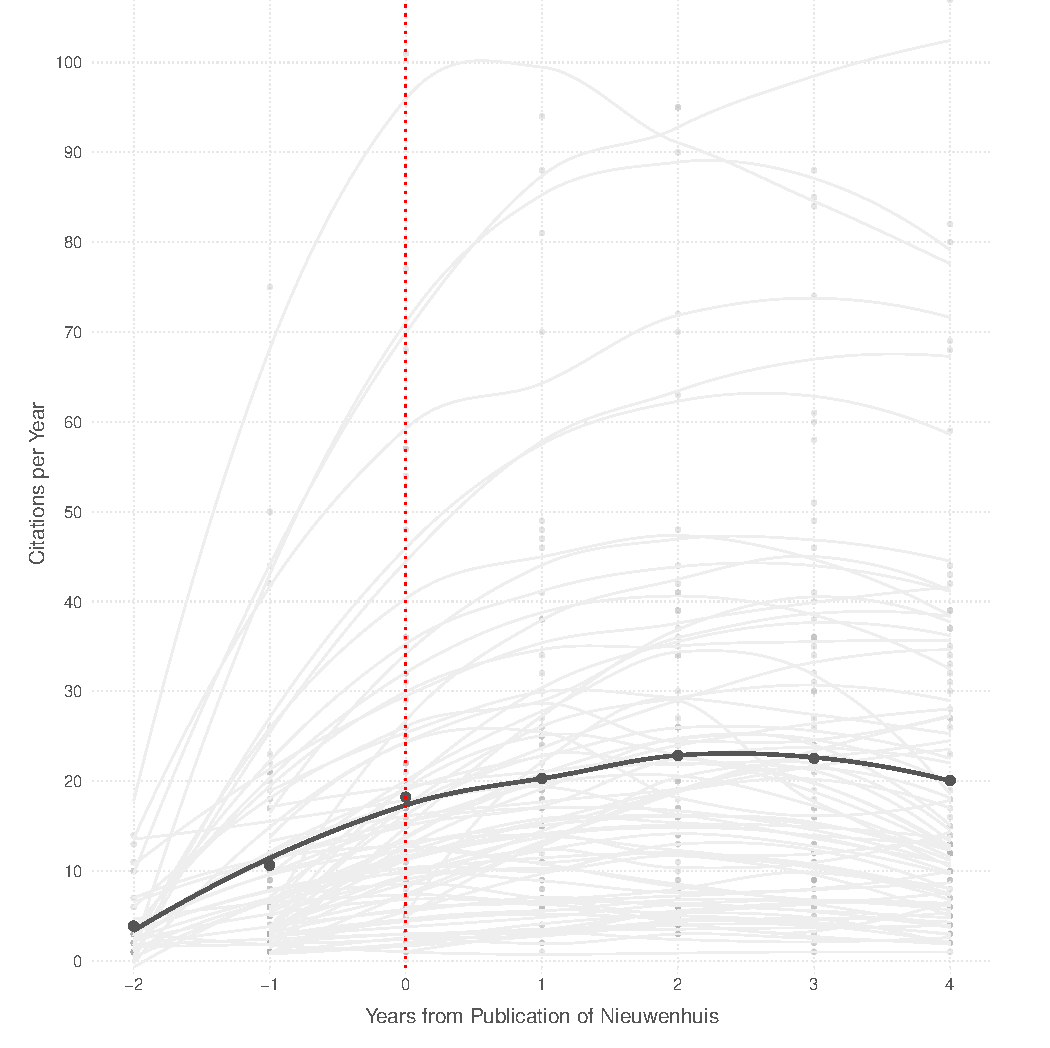
\includegraphics[scale=.7]{../figs/nw_growth_curve.pdf}
 \caption{Number of Citations to Articles Containing the Error Per Year}
 \label{fig:niewenhuis}
\end{figure}

But citations to erroneous research don't need to decline after the error in the research is publicized. We only expect approving citations to decline. To estimate how many citations after the publication of Nieuwenhuis et al. are approving, we coded whether the citation was approving or not in 100 randomly chosen articles citing articles with the mistake (see SI \ref{approving_or_not} for further details about how the citations were coded.) Of the 100, only one article noted concerns with the cited article, citing \citep{nieuwenhuis2011} for support. In all, there is strong evidence that approving citations are extremely common after the error is publicized.

To more formally explore the change in citation rate as a consequence of the publication of \citet{nieuwenhuis2011}, we started with an `event study design' focusing on the citation rates to articles with the error. We regressed citations per year on a dummy for the year \citet{nieuwenhuis2011} was published, a linear time trend, and fixed-effect for the article. We also cluster by articles to account for multiple observations per article. In effect, we are getting an average of within article changes after regressing out a linear time trend. Results show, if anything, a modest uptick in citations after \citet{nieuwenhuis2011} is published---a year after publication of \citet{nieuwenhuis2011}, articles containing the error get about four more citations per year compared to what they were getting before it (see Table \ref{tab:si_tab1}).

Our main analysis for the \citeauthor{nieuwenhuis2011} data is a Difference-in-Differences (DID) analysis. DID gives us a better way to control for over time trends, though as you will see, the results echo the results from the simpler analysis. We estimated whether the difference in citation rates of articles making the error and those not making the error changed after the publication of \citet{nieuwenhuis2011}. In particular, we regressed citations per year on whether or not the article makes the error, the year(s) after the publication of \citet{nieuwenhuis2011}, and interaction between the two. We also include fixed-effects for each article to do within article estimation. Including fixed-effects allows us to circumvent concerns around skew in citations. And we again clustered the standard errors by article.

Table \ref{tab:tab1} tabulates the results. Models (1), (3), and (5) define error as all article making the error. And Models (2), (4), and (6) refer to error as articles making ``potentially serious errors.'' As the table shows, 1 or 2 years after \citet{nieuwenhuis2011}, articles making the error were being cited more frequently vis-\`a-vis articles not making the error (Diff. $\sim$ 3). Three years out, we cannot still reject the 0, suggesting that there is no evidence of a decline. For articles making ``potentially serious errors'', the story is much the same, except that the 1 and 2-year out estimates are closer to 3.5 additional citations per year than 3. And three years later, we still cannot say that the articles making ``potentially serious errors'' were being cited any less frequently.  In all, there is strong evidence that approving citations are extremely common after the error is publicized.


% Table created by stargazer v.5.2.2 by Marek Hlavac, Harvard University. E-mail: hlavac at fas.harvard.edu
% Date and time: Fri, Aug 03, 2018 - 1:38:56 PM
% Requires LaTeX packages: dcolumn rotating 
\begin{sidewaystable}[!htbp] \centering 
  \caption{Difference-in-Difference Analysis of the Impact of Publication of Nieuwenhuis on the Number of Times per Year Articles Containing the Error Are Cited Vis-a-Vis Articles that Didn't Contain the Error} 
  \label{tab:tab1} 
\small 
\begin{tabular}{@{\extracolsep{5pt}}lD{.}{.}{-1} D{.}{.}{-1} D{.}{.}{-1} D{.}{.}{-1} D{.}{.}{-1} D{.}{.}{-1} } 
\\[-1.8ex]\hline 
\hline \\[-1.8ex] 
 & \multicolumn{6}{c}{\textit{Dependent variable:}} \\ 
\cline{2-7} 
\\[-1.8ex] & \multicolumn{6}{c}{Citations per year} \\ 
 & \multicolumn{2}{c}{1 year out} & \multicolumn{2}{c}{2 years out} & \multicolumn{2}{c}{3 years out} \\ 
\\[-1.8ex] & \multicolumn{1}{c}{(1)} & \multicolumn{1}{c}{(2)} & \multicolumn{1}{c}{(3)} & \multicolumn{1}{c}{(4)} & \multicolumn{1}{c}{(5)} & \multicolumn{1}{c}{(6)}\\ 
\hline \\[-1.8ex] 
 Treatment Date & 7.2^{***} & 7.7^{***} & 5.1^{***} & 5.5^{***} & 3.7^{***} & 3.9^{***} \\ 
  & (0.9) & (0.7) & (0.9) & (0.7) & (1.0) & (0.8) \\ 
  Error or Not & 1.5 & 0.004 & 2.1 & 0.6 & 2.8 & 1.6 \\ 
  & (2.5) & (2.8) & (2.4) & (2.7) & (2.4) & (2.6) \\ 
  Makes Error*Treatment Date & 3.1^{**} & 3.7^{***} & 2.7^{**} & 3.5^{***} & 1.7 & 2.1 \\ 
  & (1.2) & (1.3) & (1.2) & (1.3) & (1.3) & (1.5) \\ 
  Constant & 9.5^{***} & 10.2^{***} & 11.7^{***} & 12.6^{***} & 13.1^{***} & 14.0^{***} \\ 
  & (1.8) & (1.5) & (1.7) & (1.5) & (1.7) & (1.4) \\ 
 \hline \\[-1.8ex] 
Observations & \multicolumn{1}{c}{957} & \multicolumn{1}{c}{957} & \multicolumn{1}{c}{957} & \multicolumn{1}{c}{957} & \multicolumn{1}{c}{957} & \multicolumn{1}{c}{957} \\ 
Akaike Inf. Crit. & \multicolumn{1}{c}{7,328.2} & \multicolumn{1}{c}{7,327.8} & \multicolumn{1}{c}{7,408.8} & \multicolumn{1}{c}{7,407.5} & \multicolumn{1}{c}{7,474.9} & \multicolumn{1}{c}{7,475.2} \\ 
Bayesian Inf. Crit. & \multicolumn{1}{c}{7,357.4} & \multicolumn{1}{c}{7,357.0} & \multicolumn{1}{c}{7,437.9} & \multicolumn{1}{c}{7,436.7} & \multicolumn{1}{c}{7,504.0} & \multicolumn{1}{c}{7,504.4} \\ 
\hline 
\hline \\[-1.8ex] 
\textit{Note:}  & \multicolumn{6}{l}{$^{*}$p$<$0.1; $^{**}$p$<$0.05; $^{***}$p$<$0.01} \\ 
 & \multicolumn{6}{l}{Models (1), (3), and (5) define error as any article making the error.} \\ 
 & \multicolumn{6}{l}{And Models (2), (4), and (6) refer to error as articles making ``potentially serious errors.''} \\ 
\end{tabular} 
\end{sidewaystable} 


An article published in a prominent journal flagging potentially serious concerns about statistical analysis in a set of articles is one thing, a retraction notice is quite another. A majority of the articles that are retracted are retracted, as we show below, because of serious error or fraud. We expect a much stronger response to the publication of retraction notices. We expect retracted articles to \textit{never} be approvingly cited a year or more---taking account of long publication windows---after the retraction notice has been published. As we show below, the data suggests otherwise. 

Over the last thirty or so years, the number of retractions has increased sharply (see Figure~\ref{fig:n_retraction_notices_per_year}). The first retraction notice that we have in our database is from 1989. That year and the decade after it, the number of retraction notices being published per year never crossed 20. Since then, there has been a sharp and accelerating rise in the number of retraction notices per year. Between 2001, when 16 retraction notices were published, and 2015, last year for which we have complete data, there was a near 30 fold increase; a total of 451 retraction notices were published in 2015. The pattern that we find is consistent with results from \citet{steen2013has}, who also find a rapid increase in retractions over time.

\begin{figure}[H]
\centering
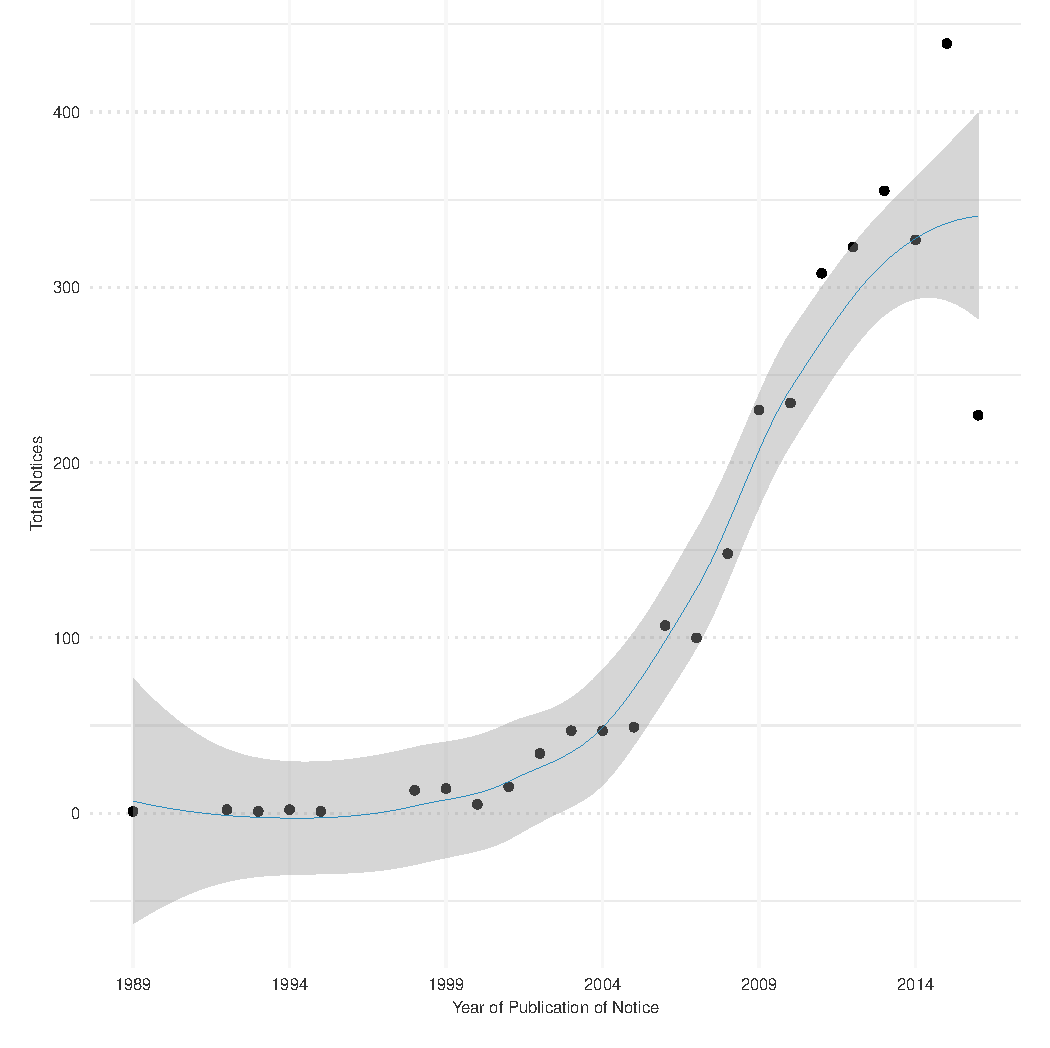
\includegraphics[scale=.7]{../figs/n_retraction_notices_by_year.pdf}
\caption{Retraction Notices Per Year}
\label{fig:n_retraction_notices_per_year}
\end{figure}

The rapid rise in the number of retractions is likely a combination of increasing production and improvements in detection. But the bottom line is that there is an ever faster growing number of articles which the scientific community thinks should not have have been published in the first place. 

These retractions are spread unevenly across disciplines. About 65.2\% of the retracted articles are from Life Sciences and Biomedicine, and 13\% are from Physical Sciences. (For a breakdown by field, see Table \ref{tab:ret_field}.) We cannot be sure about the source of the variation. It could be that the variation is entirely explained by how many articles are published in each field.

To understand why the articles are retracted, we coded a random sample of 100 retraction notices. 39\% of the notices mentioned plagiarism as one of the major reasons for retracting the article. (Plagiarism includes self-plagiarism, duplication of data, words, and publishing the same or similar article in multiple journals.) Major errors or fraud contributed to another 51\% of the retractions, with fraud alone contributing to 24\% of the retractions. Ethics violations (2) and conflict over authorship or approval from other authors (5) contributed to the rest. The percentage of retractions attributable to major errors or fraud in our data is similar to the number obtained by other research on reasons for retraction in other corpora. For instance, a study of 1,112 Biomedicine articles retracted between 1997 and 2009 found that 55\% were retracted for some type of misconduct \citep{budd2011retracted} (see also \citet{steen2010retractions}). All in all, articles are mostly retracted because the research cannot be trusted.

These flawed articles often accrue a fair number of citations before being retracted. In our data, the articles had been cited 39,792 times before being retracted. This is not unsurprising, given that it took, on average, 2.85 years for the article to be retracted. The median time before the article was retracted was two years (see Figure \ref{fig:ttr}) with 28.1\% of the articles taking 4 or more years to be retracted. These numbers are similar to those obtained elsewhere. A study on time to retraction in the PubMed corpus found that the average time to retraction was approximately three years  \citep{steen2013has}. 

\begin{figure}[H]
\centering
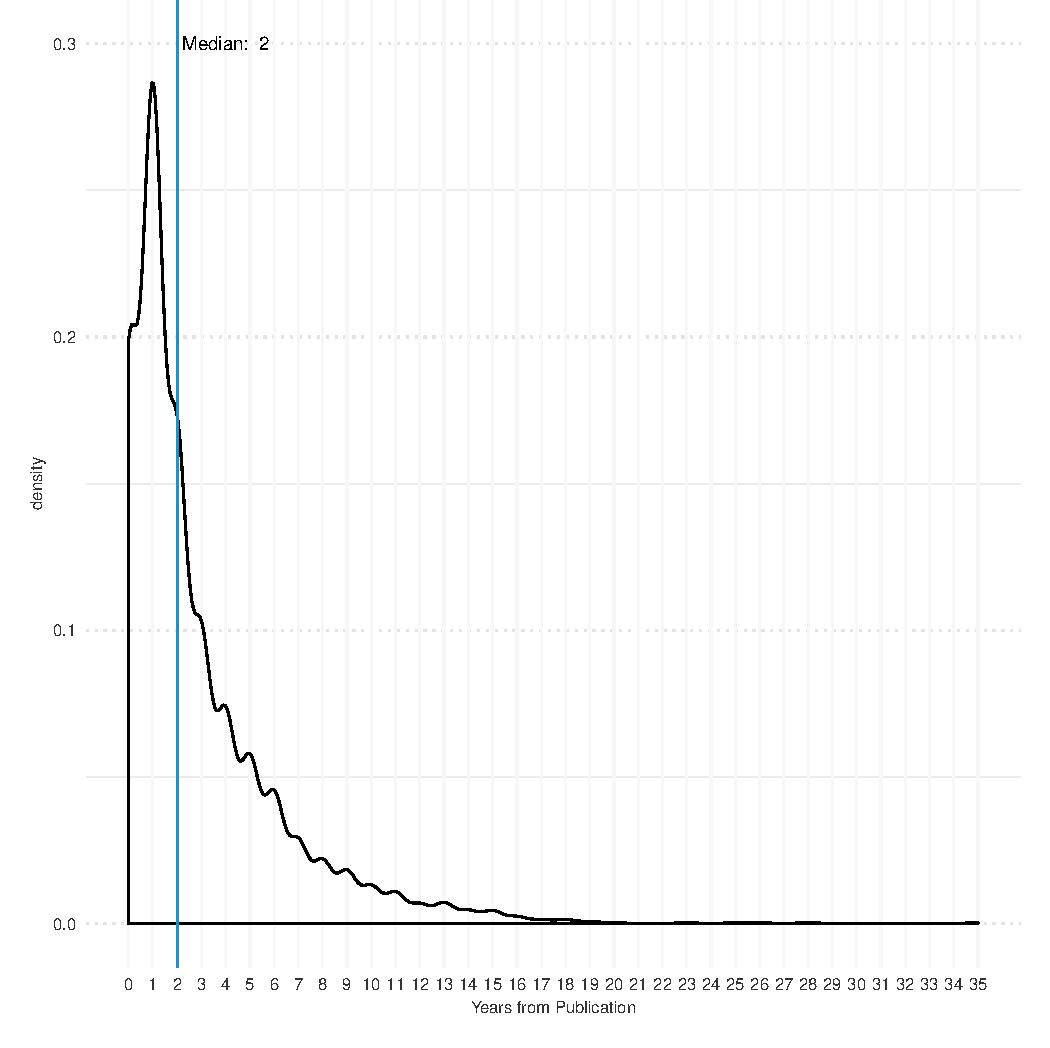
\includegraphics[scale=.7]{../figs/time_to_retraction.pdf}
\caption{Time to Retraction}
\label{fig:ttr}
\end{figure}

On the hunch that greater readership of more prominent journals would mean that problematic articles are flagged more quickly, we estimated the relationship between journal impact factor and average time to retraction. As Figure \ref{fig:jif_ttr} shows, the relationship is flat---flawed articles in low ranked journals are retracted as quickly as flawed articles in higher ranked journals.

\begin{figure}[H]
\centering
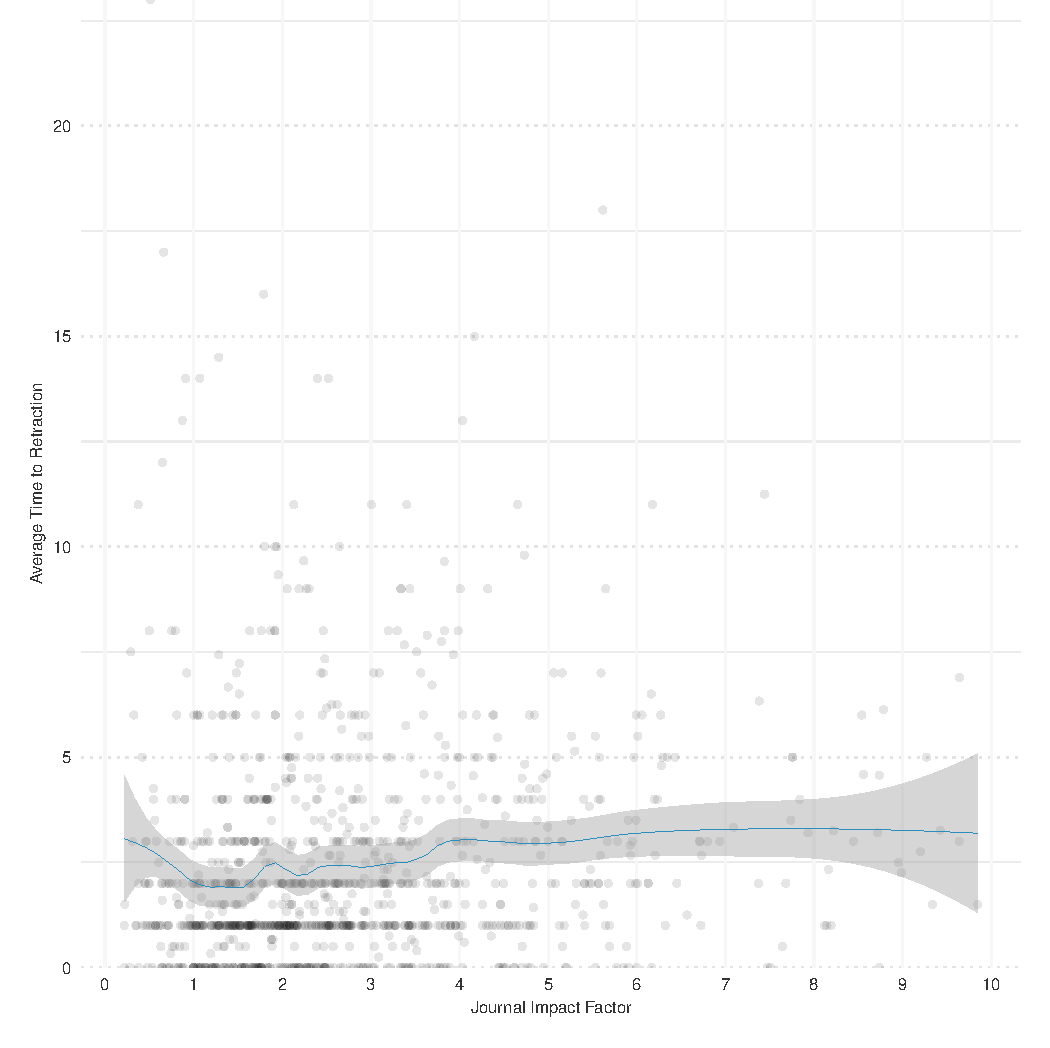
\includegraphics[scale=.7]{../figs/jif_time_to_retraction.pdf}
\caption{Relationship Between Journal Impact Factor and Time to Retraction}
\label{fig:jif_ttr}
\end{figure}

Given that a majority of retracted articles are retracted because of serious error or fraud, we expect retracted articles to \textit{never} be approvingly cited a year or more---taking account of long publication windows---after the retraction notice has been published. However, retracted articles were cited another 22,932 times between the year after they were retracted and August 2016. Thus, on average, the retracted articles received an additional 7.57 citations. Given the skew in retraction notices, with the bulk being published in recent years, these totals include very little post retraction data for many of the articles. In other words, the results are a \textit{lower bound} of the percentage of citations that happen after an article has been retracted.

To explore the frequency of citations before and after retraction, we plotted line graphs of total citations per article per year against year from the publication of retraction notice (see Figure \ref{fig:pre_post_retraction}). And we overlaid the lines with the median number of citations per article per year. We limit ourselves to 10 years before and after the publication of retraction notice as the data are very sparse beyond that. Total citations decline when the retraction notice is published---the median goes from 3 to 2 between the year retraction notice is published after next year. But the decline is followed by a plateauing.

\begin{figure}[H]
\centering
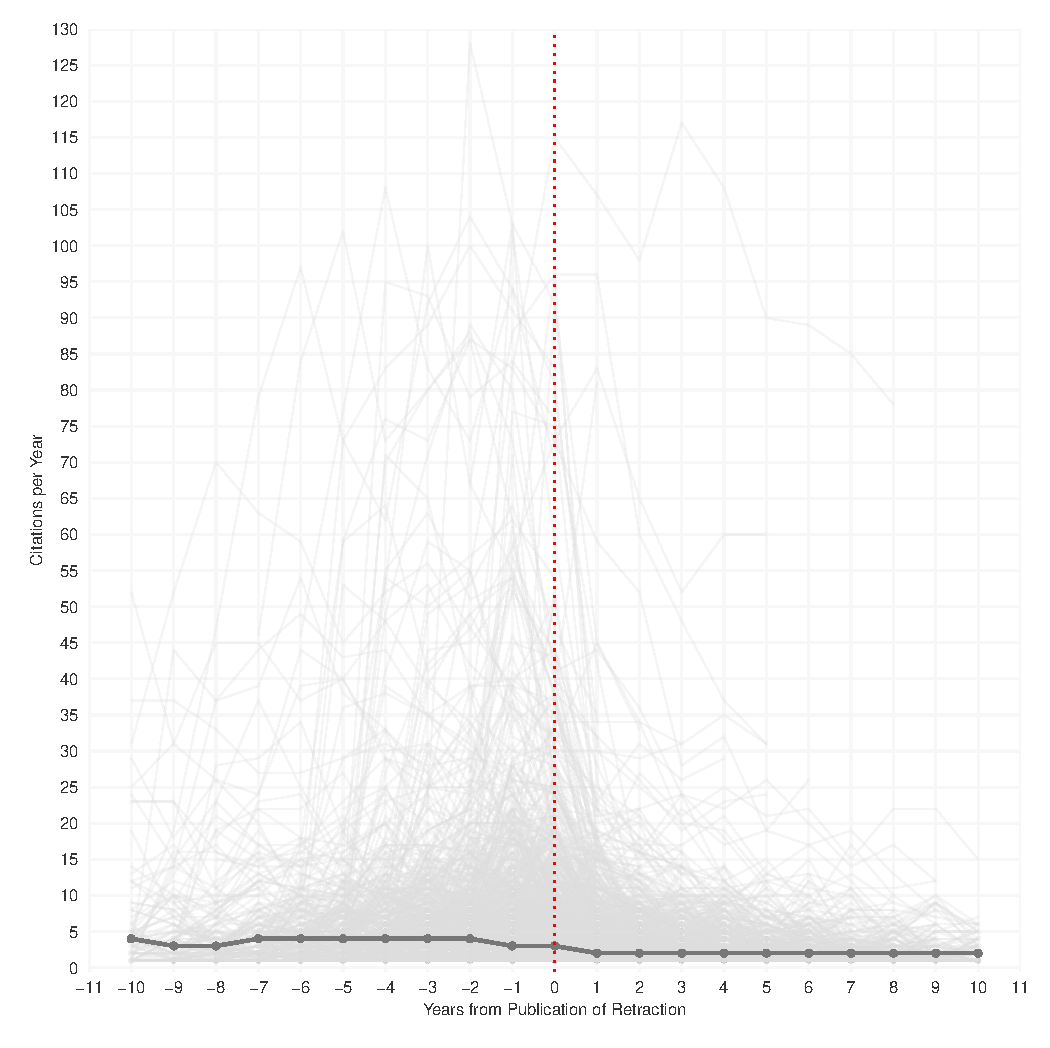
\includegraphics[scale=.7]{../figs/retracted_growth_curve.pdf}
\caption{Number of Citations to Retracted Articles per Year}
\label{fig:pre_post_retraction}
\end{figure}

Figure \ref{fig:pre_post_retraction} elides over the fact that we do not observe data on all articles after all the plotted years after the publication notice. For instance, if the retraction notice was published in 2014, we only observe one more full year of citations---2015. Thus, to look more formally at the impact of publication of retraction notices a year, 2 years, and 3 years after, we create subsets of data where we have all the articles for which we have at least 1 year, 2 years, and 3 years worth of data after the publication of the retraction notice. To analyze these subsets, we use a pretty simple model. We regress the number of citations per year per article on years from retraction notice, a dummy for the cliff (1-, 2-, and 3- years after the publication of the retraction notice) and an interaction between the two. We cluster the standard errors by article to account for the fact that we have multiple observations per article. The results of the model can be seen in Table \ref{tab:tab2}.


% Table created by stargazer v.5.2.2 by Marek Hlavac, Harvard University. E-mail: hlavac at fas.harvard.edu
% Date and time: Fri, Feb 05, 2021 - 9:49:48 AM
% Requires LaTeX packages: dcolumn 
\begin{table}[!htbp] \centering 
  \caption{Impact of Publication of Retraction Notice on the Number of Times Retracted Articles Are Cited per Year} 
  \label{tab:tab2} 
\begin{tabular}{@{\extracolsep{5pt}}lD{.}{.}{-1} D{.}{.}{-1} D{.}{.}{-1} } 
\\[-1.8ex]\hline 
\hline \\[-1.8ex] 
 & \multicolumn{3}{c}{\textit{Dependent variable:}} \\ 
\cline{2-4} 
\\[-1.8ex] & \multicolumn{3}{c}{Citations Per Year} \\ 
 & \multicolumn{1}{c}{1 Year Later} & \multicolumn{1}{c}{2 Years Later} & \multicolumn{1}{c}{3 Years Later} \\ 
\\[-1.8ex] & \multicolumn{1}{c}{(1)} & \multicolumn{1}{c}{(2)} & \multicolumn{1}{c}{(3)}\\ 
\hline \\[-1.8ex] 
 (1, 2, 3) Years After Notice & -2.4^{***} & -2.1^{***} & -1.9^{***} \\ 
  & (0.2) & (0.2) & (0.3) \\ 
  Years to Notice & -0.01 & -0.2^{***} & -0.3^{***} \\ 
  & (0.03) & (0.03) & (0.03) \\ 
  (1, 2, 3) Years After Notice*Years to Notice & -0.4^{***} & -0.2^{***} & 0.002 \\ 
  & (0.04) & (0.05) & (0.1) \\ 
  Constant & 6.0^{***} & 5.2^{***} & 4.7^{***} \\ 
  & (0.2) & (0.1) & (0.2) \\ 
 \hline \\[-1.8ex] 
Observations & \multicolumn{1}{c}{12,511} & \multicolumn{1}{c}{11,486} & \multicolumn{1}{c}{10,428} \\ 
Akaike Inf. Crit. & \multicolumn{1}{c}{83,835.6} & \multicolumn{1}{c}{76,511.3} & \multicolumn{1}{c}{69,534.9} \\ 
Bayesian Inf. Crit. & \multicolumn{1}{c}{83,880.2} & \multicolumn{1}{c}{76,555.4} & \multicolumn{1}{c}{69,578.4} \\ 
\hline 
\hline \\[-1.8ex] 
\textit{Note:}  & \multicolumn{3}{r}{$^{*}$p$<$0.1; $^{**}$p$<$0.05; $^{***}$p$<$0.01} \\ 
\end{tabular} 
\end{table} 


As Table \ref{tab:tab2} shows, on average an article is cited about 5--5.5 times per year. But 1, 2, and three years later, an average article accrues about two fewer citations per year, a drop that is statistically and substantively significant. There is also a small negative slope in the number of citations per year for models that estimate the effect 1 and two years out. So the number of citations is slowly decreasing. But note that our priors are post-retraction, articles would not be cited. So we must compare the citation rate to 0. And there we can comfortably reject the 0---citation rate post publication of the retraction notice is not zero.  

But we are being imprecise. Our claim is about approving citations---after the publication of the retraction notice, the number of approving citations should go to 0. To estimate how many of the citations are \textit{approving}, we coded a random sample of 100 articles that cited a retracted article pre-retraction and 275 articles that cited retracted research a year or more after the publication of the retraction notice. We could not locate 32 articles, leaving us with 343 articles. There were no false positives. Of the 87 articles citing retracted articles before or in the same year the retraction notice was published, 85 (97.7\%) were approving. And of the 256 articles citing retracted articles the year after the retraction notice was published, 234 (91.4\%) were approving. (Figure \ref{fig:prop_approving_per_year} plots the proportion of approving citations by year.) 

\begin{figure}
\centering
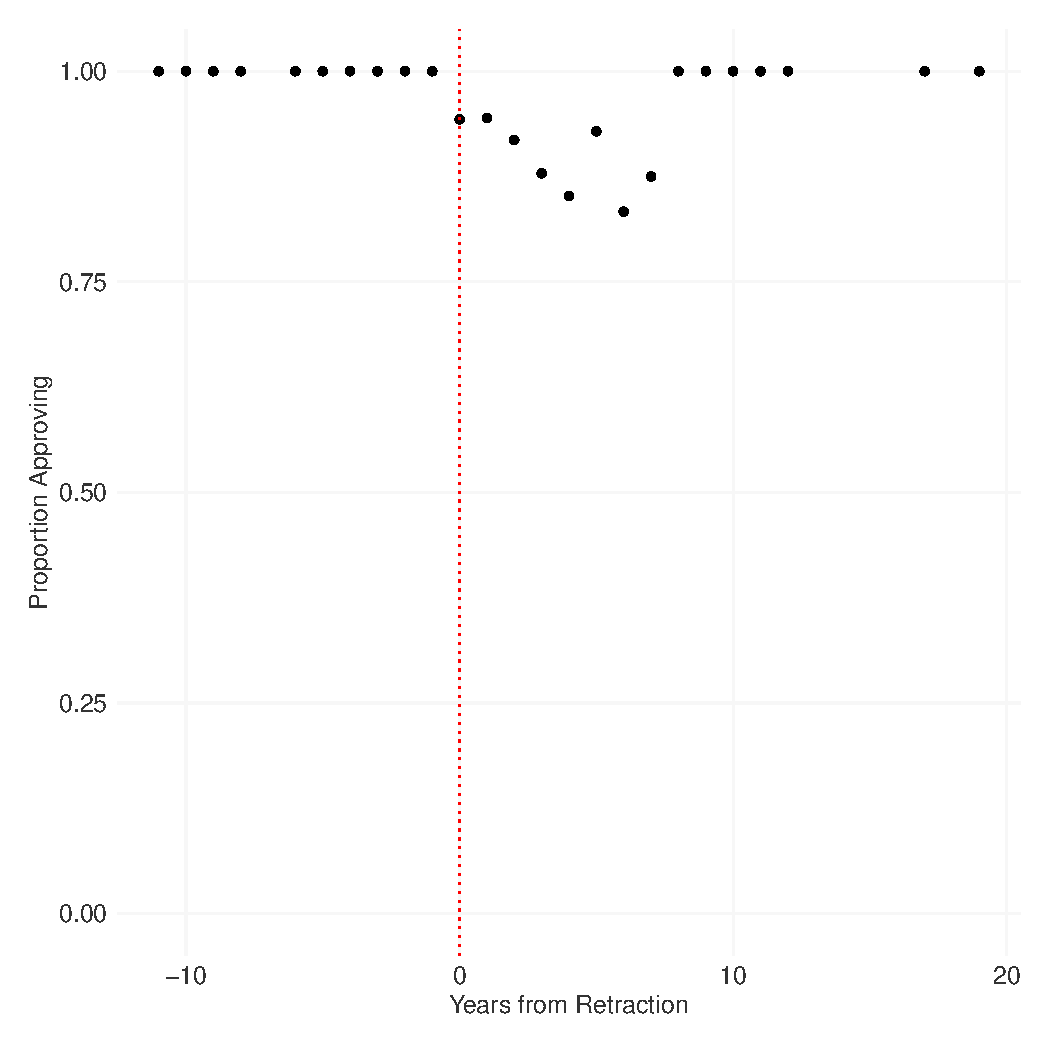
\includegraphics[width=10cm]{../figs/pre_post_prop_approving.pdf}
\caption{Proportion of Citations That Are Approving Per Year}
\label{fig:prop_approving_per_year}
\end{figure}

In all, the data suggest that retracted articles continue to be approvingly cited long after the publication of retraction notice. 

\section*{Discussion}
Only some of the points that scientists make in a paper rely on original work. Many, if not most of the points made in a typical paper, rely on work done by others. That is the nature of the scientific enterprise. But sometimes the work done by others is problematic. For instance, sometimes the claims made by the work being cited are not only wrong but made with fraudulent data. If at all scientists refer to such work, we expect scientists to acknowledge the issues carefully, especially when the errors have been publicized. We expect approving citations to problematic research to stop once the problems have been made public. But data suggest that publicizing serious errors via public retractions or publication of research highlighting the problem at prominent venues leads to, at best, a modest decline in citations. Retracted articles continue to be cited approvingly years after they have been publicly retracted.

But why do scientists fall short? We suspect that they fall short because they place too much faith in others and because they are resource constrained. Scientists sometimes do not scrutinize the article they cite because they trust the published work or trust the integrity of references in old databases or are under intense pressure to publish.

Perhaps the single most important reason why researchers approvingly cite research with serious errors, even after the errors have been publicized, is that scientists trust other scientists, especially peer-reviewed work produced by other scientists. One likely reason for that trust is the belief that scientific misconduct is limited to a few bad people. And that optimism is likely driven by the fact that a few cases of fraud get a bulk of the attention, with reporting often focusing on personalities than processes. Cases of Diederik Stapel, who fabricated data behind at least 30 papers \citep{levelt2012flawed}, John Darsee, who faked data behind nearly 100 publications \citep{stewart1987integrity, anderson2013research, wallis1983fraud}, and Jan Hendrik Sch{\"o}n, who during a period in 2001 published a research paper every 8 days based on fabricated data \citep{service2003scientific, anderson2013research}, are legend. So are cases of Andrew Wakefield, who published an article linking MMR vaccine to autism using fabricated data \citep{wakefield1998retracted, deer2011case, godlee2011wakefield}, and recently Michael Lacour, who published a paper in \textit{Science} based on fabricated data \citep{broockman2015irregularities, mcnutt2015editorial}.\footnote{Other prominent cases include that of William Summerlin, who painted mice rather than transplant skin \citep{basu2006they, anderson2013research}, Woo Suk Hwang, who claimed to have cloned embryos, Eric Poehlman, who fabricated data behind at least ten papers and numerous grant applications.} Each of these cases was framed as an example of misconduct by a bad actor, the subtext often being that a bad actor is an exception, not the rule. 

Misconduct, however, is not limited to a few bad actors.  A large anonymous survey of early- and mid-career scientists found that about 2\% of scientists admitted to engaging in fabricating, falsifying, or plagiarizing in the last \textit{three} years \citet{martinson2005scientists} (see also \citet{titus2008repairing}). Another study found that nearly 34\% of the respondents in past surveys had admitted to engaging in questionable research practices \citet{fanelli2009many}.

The other likely reason behind trust in peer-reviewed research is the fact that the rate of retractions is extremely low. For instance, of the nearly 9.4 million articles published between 1950 and 2004 and available on PubMed, only 596 have been retracted \citep{cokol2007many}. In all likelihood, however, the actual rate of serious errors in manuscripts is manifolds that rate. For instance, \citet{cokol2007many} estimate the rate at which articles ought to be retracted to be anywhere between 16.7 times to 167.8 times the actual rate. And these estimates do not account for research that involves harder-to-prove malpractice such as stuffing non-significant results in the file-drawer \citep{franco2014publication}, conducting specification searches, and other more fundamental concerns like low power, which reduces the likelihood that a nominally statistically significant finding reflects a true effect \citep{button2013power, ioannidis2005most}. All in all, while the belief that most research that is produced is reliable is very likely unfounded, it probably explains why scientists approvingly cite erroneous research. 

According to us, the second biggest reason why scientists cite erroneous research is lack of time. Given the pressure to publish, many researchers likely do not spend enough time vetting the research they cite. Pressed for time, scientists often likely default to credulousness when evaluating the research they cite. There is also likely some `motivated vetting,' with articles cited in `support' likely receiving less scrutiny than those making the `opposing' argument. 

Thirdly, incentives to cite carefully are mostly absent. More often than not, the only thing researchers are ever knocked on when it comes to citations is failing to cite someone or missing the journal's formatting requirements. Citing incorrectly or citing bad research flatteringly generally attracts little opprobrium.  

Fourthly, when researchers are searching for relevant research, there are no tools that reliably alert researchers about errors in research. At the time of writing, Google Scholar, for instance, does not flag if an article has been retracted, much less flag articles that have found serious problems with the article.

Lastly, often, researchers rely on old reference databases sitting on their computer for citations. And researchers likely don't check if these databases contain articles that have since been retracted because of the reasons we discuss above---chances are low. For instance, \citet{davis2012persistence} finds that personal Mendeley libraries contained 1,340 retracted articles. All in all, there are a lot of reasons to suspect that scientists would cite erroneous research, even when errors have been publicized via the publication of a retraction notice or an article noting the problem.

These `mistakes'---citing flawed research when flaws have been made public---are avoidable. Assuming that researchers do not knowingly approvingly cite retracted articles, the data imply that the discovery of errors, even when public retraction notices are issued, is still a problem. 

To ameliorate the problem, we need to improve access to information about problems in research. One way to improve access to information about problems is to build tools that provide the information as part of existing research discovery and production processes. For instance, altering interfaces of heavily used portals such as Google Scholar, JSTOR, journal publishers' sites, etc. so that they thread reproduction attempts, retractions, and other research that directly bears on the evidence presented in an article along with the article are liable to be effective. Rather than effect change in multiple interfaces, which requires coordination with multiple strategic actors, however, a better strategy may be to create a browser plug-in that highlights problematic articles listed on a web page. Providing such a tool to editors or copy editors at academic publishers may also help ameliorate the problem. Flagging problems during the scientific discovery process, however, is better than flagging them during the production process. Flagging during discovery likely preempts the temptation to engage in post hoc rationalization. Alternately, one could build tools that automatically create pull requests to personal bibliography libraries posted on open publication platforms like GitHub. Lastly, while our study only tallies research that cites known flawed research, it is quite likely that the effect of flawed research extends to studies that cite studies that approvingly cite flawed research (and thereon).  And any modifications to the interface should extend to papers that cite flawed research so that people citing them, in turn, are also warned. 

Egregious errors like approving citations to flawed research after the flaws have been made public serve to highlight more significant problems with how science is practiced. Scholars do not appear to carefully vet research they cite. To improve the reliability of scientific production, besides innovating on better tools, we may also need also to penalize research that makes such errors.

  

\clearpage
\bibliographystyle{apsr}
\bibliography{error}

\clearpage
\appendix
\renewcommand{\thesection}{SI \arabic{section}}
\renewcommand\thetable{\thesection.\arabic{table}}  
\renewcommand\thefigure{\thesection.\arabic{figure}}
\counterwithin{figure}{section}
\setcounter{figure}{0}
\setcounter{section}{0}
\setcounter{table}{0}

\begin{center}
\Large{Supporting Information}
\end{center}

\section{Creating the Retractions Dataset}
\label{data_collection}

To build a database of retracted articles, we started by creating a list of retraction notices. To do that, in August 2016, we searched WoS for titles containing the phrase ``retraction of.'' The search yielded more than 14,000 records. Using the ``corrections'' filter in WoS---it is a WoS flag for retraction and correction notices---we filtered the list to 4,085 retraction notices.

Next, we wrote software to automatically search the WoS database for retracted articles using the information in the retraction notice records. Retraction notice records did not contain consistent titles to allow us to a simple search. But 99\% of the retraction notices contained the year the original article was published, and 96\% listed the authors of the original work. We used these two pieces of information along with the name of the publication to search the WoS for the original articles. The search resulted in a list of 3,776 articles. We could not locate the remaining 309 retracted articles.

Due to the variability in the information contained in the retraction notice records, the automated search process returned the wrong article in some cases. Our aim was to have zero false positives even at the risk of some false negatives. With that aim, we created rules to flag potential false positives. First, if the list of authors of the retracted article did not match the list of authors for the relevant retraction notice record, we flagged the record as a potential false positive. Second, if the title of the retracted article did not contain the words ``retracted'' or ``retraction,'' we flagged it as a potential false positive. (It is standard practice for titles of original articles to be revised to indicate that the article has been retracted.) Third, we parsed the title of the retracted notices to extract the title of the original retracted article. And we flagged articles where the titles did not match as potential false positives. We then reviewed the potential false positives, filtering out all records where we could not verify the match. This resulted in a set of 3,084 articles. Finally, we checked for duplicates. We found 55. This left us with 3,029 articles. And that served as our final sample. 

As an additional robustness check, we manually checked a random sample of 100 retracted articles to confirm that the article had indeed been retracted. We found that all of them were.

To get a list of citations to these articles, we used the WoS functionality that allows users to access the list of citations to articles. We wrote software to automatically download citation records for each of the retracted articles. In total, we found 73,564 citations.
\clearpage

\section{Classifying Citations as Post-Retraction or Not}
\label{pre_post}
A few retraction notices, retracted articles, and articles citing the retracted articles have earlier online (or conference) publication dates than the print publication dates recorded by WoS. As a result, post-retraction citations can be classified as otherwise. Or vice versa. To determine the impact of this issue and issues like these on our estimate of the lower bound of the proportion of citations that are made a year or more after the publication of the retraction notice, we manually recorded the online publication dates for a random sample of 300 citations to retracted articles, the associated retraction notices, and retracted articles. We could not retrieve 20 articles citing a retracted article.  Of the remaining 280 records, switching to online publication dates suggests that three articles were misclassified as post-retraction (2.2\%) and four were misclassified as not post-retraction (3.2\%). Taking these error rates at their face value, we re-calibrated our results. The recalibration results in an increase in the number of post-retraction citations, from 22,932 to 23,289. Or, the lower bound of the proportion of citations that happen the year after the retraction notice is published goes from 31.2\% to 31.7\%.

\clearpage
\section{Retracted Articles by Field}
\label{ret_art_by_field}
To understand the kinds of fields where retractions are more common, we used an augmented Web of Science research field categorization scheme to classify the articles. There is one caveat. Sometimes papers cover more than one topic. We just choose the first topic in these cases taking it to be the primary topic. 

As Table ~\ref{tab:ret_field} shows, 65\% of the retracted articles were published in the Life Sciences and Biomedicine field.  A distant second at 13\% is Physical Sciences, followed by Technology at 10.7\%. Social Sciences are at 5.5\%.  One reason why a large majority of the retractions are from the  Life Sciences and Biomedicine field may be simply because the field has more publications. But we cannot say anything definitely.

% latex table generated in R 3.5.1 by xtable 1.8-2 package
% Sun Aug 05 19:57:13 2018
\begin{table}[!htb]
\centering
  \caption{Retraction Notices By Field}
\begin{tabular}{lrr}
  \hline
Field & Number of Notices & Percentage of Total \\ 
  \hline
Arts \& Humanities & 13 & 0.4 \\ 
  Life Sciences \& Biomedicine & 1974 & 65.2 \\ 
  Multidisciplinary & 157 & 5.2 \\ 
  Physical Sciences & 393 & 13.0 \\ 
  Social Sciences & 165 & 5.5 \\ 
  Technology & 325 & 10.7 \\ 
   \hline
\end{tabular}
\label{tab:ret_field}
\end{table}


\clearpage
\section{Coding Citations as Approving or Not}
\label{approving_or_not}

To code the citations, we downloaded citing articles and their associated retracted article. A research assistant then edited the citing article pdf to highlight where the retracted article was discussed in the citing article. The judgment of whether the article noted any concerns was made based on a review of the original retracted article pdf and the highlighted text. 

If an article did not note any concerns with the cited article, it was coded as \textit{approving}. Simply disagreeing with the conclusions of an article without noting any concern still meant that the article was being cited in a way that suggests that its findings are trustworthy and were also coded as \textit{approving}. We code articles that note any concern with the citing article, even those unrelated to the cause of retraction, as \textit{disapproving}. 

In the Nieuwenhuis data, we could not locate one of the 100 articles, leaving us with 99 articles. Of the 99 articles, 2 were false positives---the articles did not cite erroneous research, but instead cited a paper with authors and title similar to published erroneous research. Of the 97 remaining articles, only one article noted concerns while citing an article making a mistake, citing \citet{nieuwenhuis2011} for support. 

In the retracted article data, we could not locate 32 articles, leaving us with 343 articles. There were no false positives. Of the 87 articles citing retracted articles before or in the same year the retraction notice was published, 85 (97.7\%) were approving. And of the 256 articles citing retracted articles the year after the retraction notice was published, 234 (91.4\%) were approving.

We evaluated the reliability of the coding by having an independent rater code 50 randomly selected citing articles. The two sets of independent codes were found to agree in all 50 instances.
\clearpage

\section{Rate of Citations Before and After Publication of Nieuwenhuis et al.}

\begin{figure}[H]
\centering
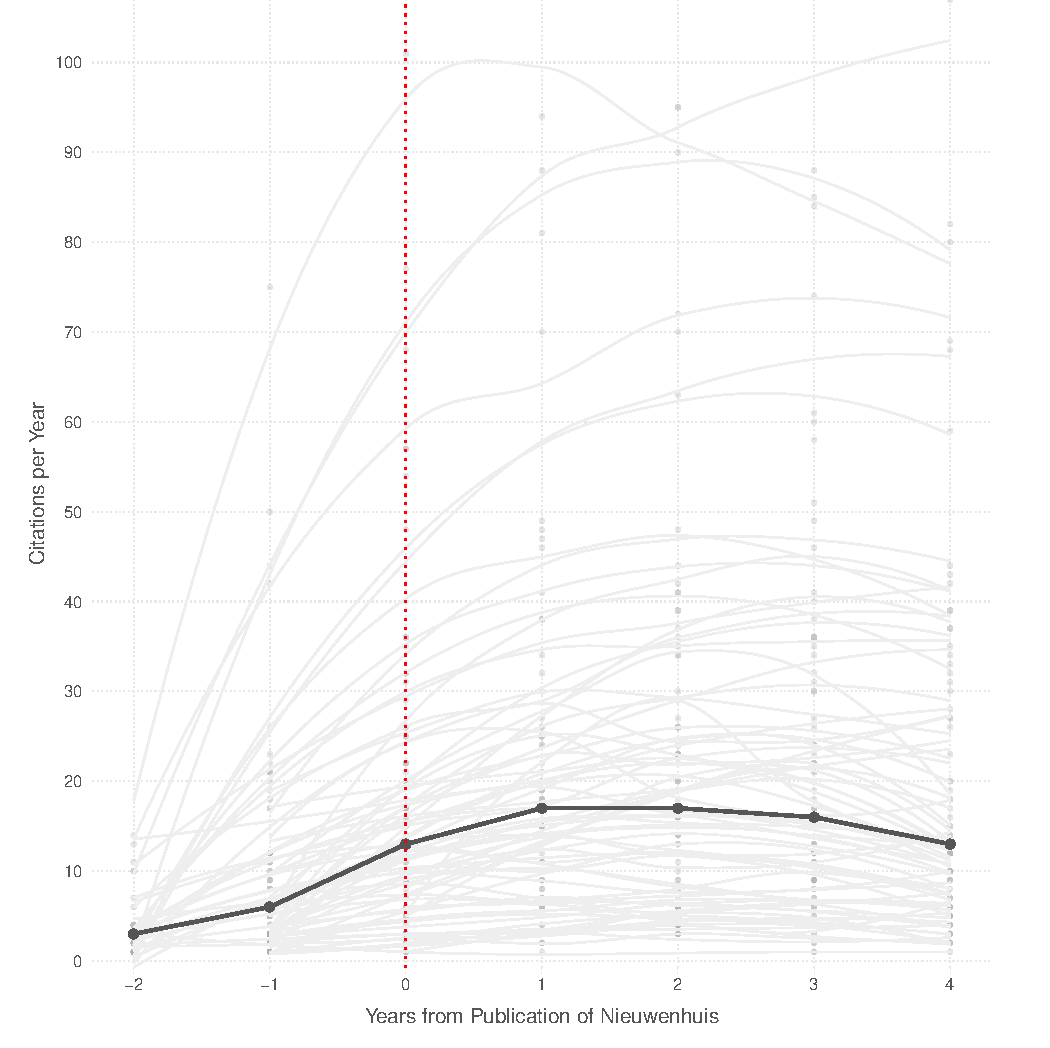
\includegraphics[scale=.7]{../figs/nw_median_growth_curve.pdf}
\caption{Total number of citations received per year by each of the papers making the mistake, and the median number of citations received per year by the articles.}
\label{fig:median_niewenhuis}
\end{figure}

\clearpage
\begin{figure}[H]
\centering
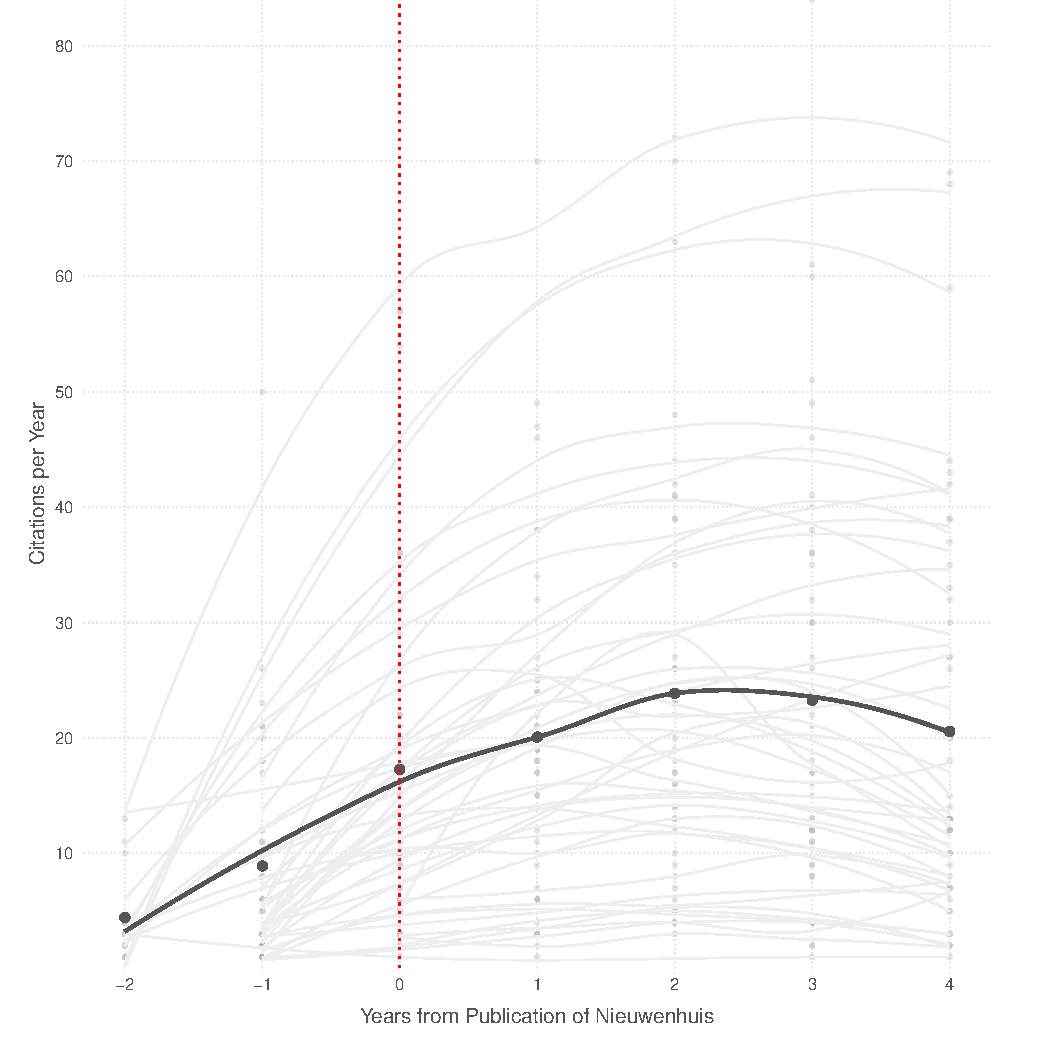
\includegraphics[scale=.7]{../figs/serious_nw_growth_curve.pdf}
\caption{Total number of citations received per year by articles making the mistake with `potentially serious' consequences for the results, and the average number of citations received per year by the articles.}
\label{fig:serious_niewenhuis}
\end{figure}

\clearpage

% Table created by stargazer v.5.2.2 by Marek Hlavac, Harvard University. E-mail: hlavac at fas.harvard.edu
% Date and time: Fri, Aug 03, 2018 - 1:38:47 PM
% Requires LaTeX packages: dcolumn 
\begin{table}[!htbp] \centering 
  \caption{Change in the Number of Citations to Articles Containing the Error Per Year Before and After Publication of Nieuwenhuis} 
  \label{tab:si_tab1} 
\begin{tabular}{@{\extracolsep{5pt}}lD{.}{.}{-1} D{.}{.}{-1} } 
\\[-1.8ex]\hline 
\hline \\[-1.8ex] 
 & \multicolumn{2}{c}{\textit{Dependent variable:}} \\ 
\cline{2-3} 
\\[-1.8ex] & \multicolumn{2}{c}{Citations Per Year} \\ 
 & \multicolumn{1}{c}{All Articles with Mistakes} & \multicolumn{1}{c}{Articles with Potentially Serious Errors} \\ 
\\[-1.8ex] & \multicolumn{1}{c}{(1)} & \multicolumn{1}{c}{(2)}\\ 
\hline \\[-1.8ex] 
 Transition Date & 3.8^{**} & 5.0^{**} \\ 
  & (1.7) & (2.0) \\ 
  Time & 2.0^{***} & 2.1^{***} \\ 
  & (0.4) & (0.5) \\ 
  Constant & 12.4^{***} & 11.6^{***} \\ 
  & (1.9) & (2.1) \\ 
 \hline \\[-1.8ex] 
Observations & \multicolumn{1}{c}{487} & \multicolumn{1}{c}{276} \\ 
Akaike Inf. Crit. & \multicolumn{1}{c}{3,818.0} & \multicolumn{1}{c}{2,095.8} \\ 
Bayesian Inf. Crit. & \multicolumn{1}{c}{3,838.9} & \multicolumn{1}{c}{2,113.9} \\ 
\hline 
\hline \\[-1.8ex] 
\textit{Note:}  & \multicolumn{2}{r}{$^{*}$p$<$0.1; $^{**}$p$<$0.05; $^{***}$p$<$0.01} \\ 
\end{tabular} 
\end{table} 


\end{document}
